\documentclass[main.tex]{subfiles}
\begin{document}

\section{Grammatical Relations}

The simplest classification approach used in this study considered the relative frequency of different grammatical relations. For this approach, the governor and the dependent of the dependencies were ignored, with only the relation itself being used. 

Each data set instance contained attributes corresponding to dependency relations. The Stanford parser system in its default configuration does not generate the \textit{punct} or punctuation dependency which connects punctuation symbols to a key element in the associated clause. Since English punctuation is broadly similar to Spanish punctuation, aside from some stark differences such as Spanish's inverted question and exclamation marks, which should be apparent to even the beginning learner, it did not seem to useful to activate this dependency. Additionally, the \textit{abbrev} or abbreviation dependency was removed. This dependency marks the definition of an abbreviation, as in the example given by \citet{typed-deps-manual}, ``Australian Broadcasting Corporation (ABC),'' where the dependency would be $abbrev(\text{Corporation},\text{ABC})$. This dependency has little to do with grammar, and thus was ignored for the purposes of this study. Having excluded these two dependencies, each data set instance contained 58 numerical attributes, one for each relation used.

      For each attribute $A_r$ corresponding to the relation $r$, the corresponding value was the floating point number $n_r/n_t$, where $n_r$ and $n_t$ were the number of occurrences of the relation $r$ and the total number of relations in the text, respectively. A C4.5 decision tree classifier trained on these instances produces the decision tree shown in Figure~\ref{fig:c4.5-dep-tree}, employing 15 different relations. The full names for these relations are shown in Table~\ref{table:reln-abbr}. At each terminal node of the tree there is an integer or pair of integers in parentheses. These values indicate the number of the training cases that were categorized (correctly or not) at that node and the number of cases incorrectly categorized, this latter value only being shown when greater than zero. For any given test node, one can identify one branch as the predominately \textit{en} branch and the other as the \textit{es} branch. For test nodes where one or both branches lead to terminal nodes, this is trivial, as the terminal nodes themselves label the branches. For any other test node, the branches can be identified by summing up the number of test cases at the terminal nodes of that branch. For instance, the root test node, which considers the relation \textit{nn}, divides the training set of 642 cases into a subset of 337 cases, associated with the left branch, and another subset of 305 cases, associated with the right branch. Looking at the left branch, it can be seen that of these 336 cases, 301 of them are nonnative, i.e. of the class \textit{es}, and only 36 are native. This indicates that this is a predominately nonnative branch. Conversely, the right hand branch consists of 205 native cases and only 20 nonnative cases, making it the native branch. This allows one to say, for instance, that fewer occurrences of the \textit{nn} relation are associated with nonnative samples. The following subsections explore the linguistic reasons why these relations should be so useful in making such categorizations.

\begin{figure}[htbp]
\centering
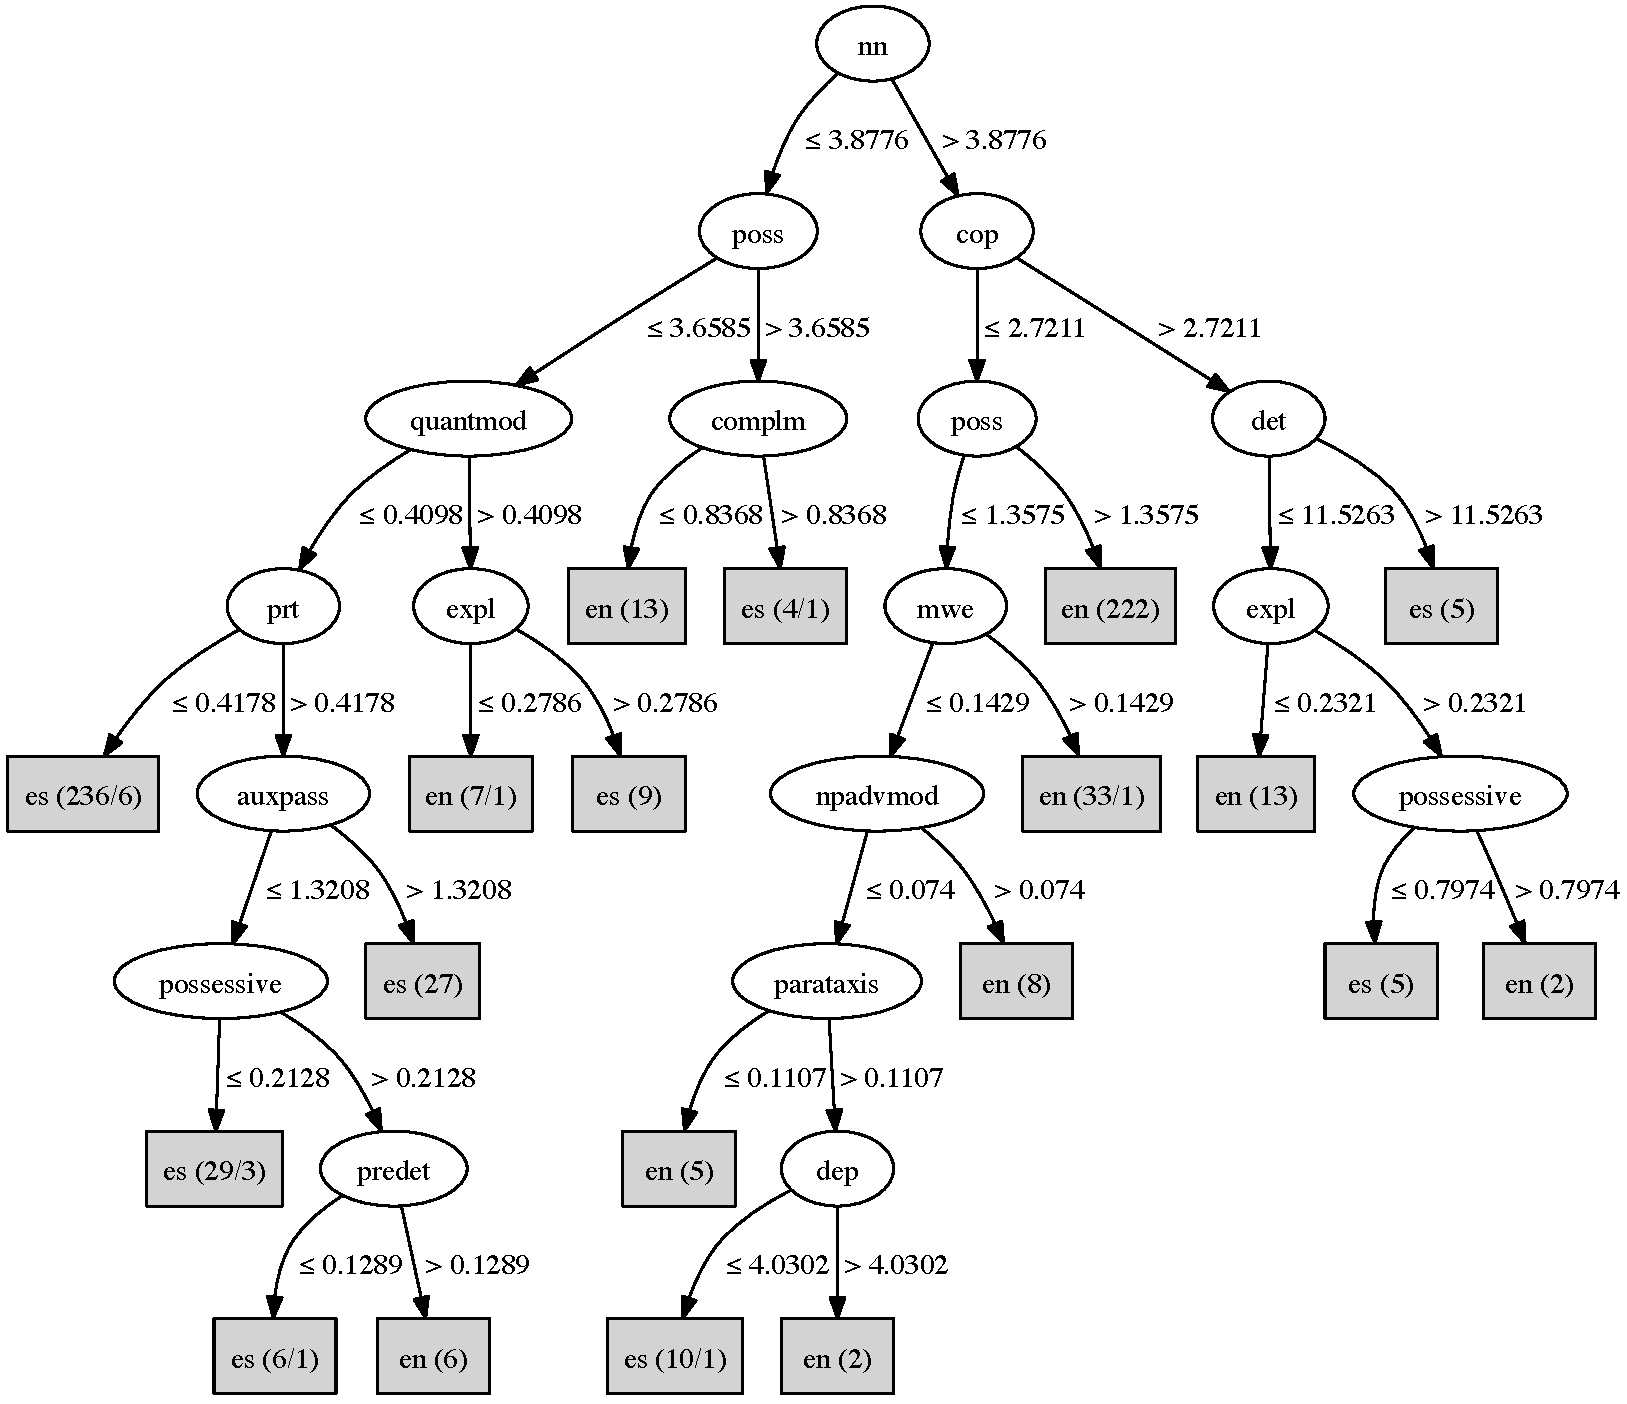
\includegraphics[width=6in]{c45-dep-graph.pdf}
\caption{C4.5 decision tree employing relative frequency of dependency relations. Relative frequencies are shown as percentages. Values in parentheses are the number of training case classified at that point and, following the slash when present, the number of those cases which were incorrectly classified.}
\label{fig:c4.5-dep-tree}
\end{figure}

\begin{table}[ht]
\small
\centering
\caption{Relation abbreviations}
\begin{tabular}{ l  l }
    \toprule
$auxpass$ & passive auxiliary \\
$complm$ & complementizer \\
$cop$ & copula \\
$det$ & determiner \\
$expl$ & expletive\\
$mwe$ & multi-word expression \\
$nn$ & noun compound modifier \\
$npadvmod$ & noun phrase as adverbial modifier \\
$parataxis$ & parataxis \\
$poss$ & possession modifier \\
$possessive$ & possessive modifier \\
$predet$ & preconjunct \\
$prt$ & phrasal verb particle \\
$quantmod$ & quantifier phrase modifier \\
$rel$ & relative \\
\bottomrule
\end{tabular}
\label{table:reln-abbr}
\end{table}


\subsection{Passive Auxiliary}

The passive auxiliary dependency \textit{auxpass} marks an auxiliary verb which carries the passive information of the clause. In general a parsed sample of text will contain one such dependency for every passive clause and so a high relative frequency of this relation indicates heavy usage of the passive voice. Figure~\ref{ex:auxpass-dep} illustrates this dependency.

\begin{figure}
\centering
\begin{tabular}{ l l }
a. & \xytext{
\xybarnode{Kennedy} &
\xybarnode{has} &
\xybarnode{been} &
\xybarnode{killed}
\xybarconnect(U,U){-1}"_{\small auxpass}"
}\\
b. & \xytext{
\xybarnode{Kennedy} &
\xybarnode{was/got} &
\xybarnode{killed}
\xybarconnect(U,U){-1}"_{\small auxpass}"
}
\end{tabular}
\caption{The dependencies $auxpass(\text{killed},\text{been})$ and $auxpass(\text{killed},\text{was/got})$. Taken from \citet{typed-deps-manual}.}
\label{ex:auxpass-dep}
\end{figure}

The decision tree in Figure~\ref{fig:c4.5-dep-tree} uses the $auxpass$ attribute once, dividing the training set into cases with higher frequencies, which get classified immediately as nonnative, and cases with lower frequencies, which undergo addition testing. It is important to note that the large majority of this second set of cases (35 out of 41) are ultimately categorized as nonnative as well. So while high relative frequencies of the $auxpass$ attribute are associated with learners, low frequencies are associated with both learners and native speakers. This indicates that the use of the passive is not a strong indicator the nativeness of the text. Likely a slightly more aggressive pruning factor would have resulted in the elimination of the $auxpass$ node.

\subsection{Complementizer}

A complementizer is a word that signals the beginning of a clausal complement. The Stanford Parser recognizes the complementizers \textit{that} and \textit{whether} as shown in Figure~\ref{ex:complm3}. The governor of a complementizer dependency is the root of the clause, which is generally a verb or, in the cause of copular clauses, the subject complement. The dependent is the complementizer itself.


\begin{figure}[ht]
\centering
\begin{tabular}{ l l }
a. &
\xytext{
\xybarnode{\ldots} &
\xybarnode{I} &
\xybarnode{will} &
\xybarnode{consider} &
\xybarnode{\ldots} &
\xybarnode{whether} &
\xybarnode{the} &
\xybarnode{world} &
\xybarnode{is} &
\xybarnode{a} &
\xybarnode{safe} &
\xybarnode{place}
\xybarconnect(U,U){-6}"_{\small complm}"
}\\

b. &
\xytext{
\xybarnode{At} &
\xybarnode{least} &
\xybarnode{you} &
\xybarnode{choose} &
\xybarnode{whether} &
\xybarnode{to} &
\xybarnode{go}
\xybarconnect(U,U){-2}"_{\small complm}" &
\xybarnode{to} &
\xybarnode{a} &
\xybarnode{pub} &
\xybarnode{or} &
\xybarnode{not.}
}\\

c. &
\xytext{
\xybarnode{They} &
\xybarnode{state} &
\xybarnode{that} &
\xybarnode{climate} &
\xybarnode{generally} &
\xybarnode{predicts}
\xybarconnect(U,U){-3}"_{\small complm}"&
\xybarnode{that} &
\xybarnode{temperatures} &
\xybarnode{should} &
\xybarnode{rise}
\xybarconnect(U,U){-3}"_{\small complm}"&
\ldots
}
\end{tabular}
\caption{The dependencies $complm(\text{place},\text{whether})$, $complm(\text{go},\text{whether})$ $complm(\text{predicts},\text{that})$, and $complm(\text{rise},\text{that})$. Nonnative samples from WRICLE (\textit{a} and \textit{c}) and SULEC (\textit{b}).}
\label{ex:complm3}
\end{figure}


\citet{whitley:1986} points out that while English tends to allow complementizers introducing clausal complements in the object position to be deleted, Spanish generally does not (see Example~\ref{ex:complm}). \citet[33.4.6]{butt} explain that this rule is occasionally broken, but generally only in two situations: business letters and substandard speech, and when the complementizer \textit{que} appears close to other uses of the word \textit{que}. Since these are restricted cases, it is reasonable to conclude that there would be L1-transfer in the construction of clausal complements, leading L1-Spanish learners to have some preference for Example~\ref{ex:complma} over \ref{ex:complmb}, particularly considering that they are both perfectly valid constructions.

In a study on differences in complement clause usage between native and nonnative English speakers, \citet{biber:1998} make a number of conclusions relevant to the current study. First, they consider when native speakers omit the complementizer \textit{that} and conclude that it is rarely omitted in academic prose and in opinion and descriptive essays. Since the vast majority of the corpus samples both native and nonnative fall into these categories, this provides encouraging evidence that the differences in complementizer usage identified by the classifier are not due to idiosyncrasies in the samples. Next, while considering four different groups of L1-speakers, French, Spanish, Chinese, and Japanese, \citeauthor{biber:1998} find that all groups shows similar levels of \textit{that} omission, and in general these levels of omission are lesser than the levels found in comparable types of native texts. They also find, interesting that L1-Spanish speakers use complement clauses, with and without omission of the complementizer, more often than either native speakers or the other groups of learners.

The decision tree shown in Figure~\ref{fig:c4.5-dep-tree} uses the $complm$ dependency once, and classifies cases with lower occurrences of $complm$ as native and larger occurrences as nonnative, without further testing. This this dependency does not part necessarily indicate the presence of a complement clause, but rather the presence of a complementizer, the higher frequency among the learners may be due either to low rates of dropping the complementizer, or high rates of complement clause usage. As shown above, both phenomena have linguistic backing and very likely both are at play. 


\begin{figure}
\eenumsentence{
\label{ex:complm}
\item \textit{I say that he'll do it.} \label{ex:complma}
\item \textit{I say he'll do it.} \label{ex:complmb}
\item \textit{Digo que lo hará.}
\item \textit{*Digo lo hará.} (\citealt[p. 278]{whitley:1986})
}
\end{figure}

\subsection{Copula}

The copula or $cop$ dependency marks copular verbs. This dependency takes as its governor the complement of the copular clause, and the verb itself as the dependent. Figure~\ref{ex:cop1} shows examples of two different copular verbs.
\begin{figure}[ht]
\centering
\begin{tabular}{ l l }
a. &
\xytext{
\xybarnode{The} &
\xybarnode{country} &
\xybarnode{became} &
\xybarnode{totally} &
\xybarnode{independent.}
\xybarconnect(U,U){-2}"_{\small cop}"
}\\

b. &
\xytext{
\xybarnode{He} &
\xybarnode{was,} &
\xybarnode{however,} &
\xybarnode{very} &
\xybarnode{interested}
\xybarconnect(U,U){-3}"_{\small cop}" &
\xybarnode{in} &
\xybarnode{my} &
\xybarnode{proposals.}
}\\
\end{tabular}
\caption{The dependencies $cop(\text{independent},\text{became})$ and $cop(\text{interested},\text{was})$. \citep[Ch. 2.15, 2.16]{quirk:1985}.}
\label{ex:cop1}
\end{figure}
However, the Stanford parser does not recognize all copular clauses as such. In particular, copular clauses followed by adverbials are not identified with the $cop$ dependency, for instance:
\enumsentence{\textit{I have been in the garden.} \citep[Ch. 2.16]{quirk:1985}}

The decision tree in Figure~\ref{fig:c4.5-dep-tree} contains one node which uses the $cop$ dependency. This node divides the training set into two subsets such that the first, associated with lower frequencies of $cop$, contains a smaller percentage of nonnative texts, and the second, with higher frequencies of the attribute, contains a larger percentage. The simplest explanation for this is simply that copular clauses tend to be the simplest type of clauses in language and thus are favored by learners. A detailed treatment of both of these points can be found in a study by \citet{hinkel:2003}, which investigates sentential simplicity in L1 and L2 academic texts.

\subsection{Determiner and Predeterminer}

The determiner or $det$ dependency connects a determiner to the NP it modifies with the determiner being the dependent and the head of the NP the governor. Similarly, the $predet$ dependency marks a predeterminer. Figure~\ref{ex:det} shows examples of both determiners and a predeterminer in one sentence fragment. 
\begin{figure}[ht]
\centering
\xytext{
\xybarnode{For} &
\xybarnode{some} &
\xybarnode{people}
\xybarconnect(U,U){-1}"_{\small det}" &
\xybarnode{to} &
\xybarnode{make} &
\xybarnode{such} &
\xybarnode{a} &
\xybarnode{fuss}
\xybarconnect(U,U){-1}"_{\small det}"
\xybarconnect(D,D){-2}"^{\small predet}" &
\xybarnode{about} &
\xybarnode{this} &
\xybarnode{matter}
\xybarconnect(U,U){-1}"_{\small det}" &
\xybarnode{\ldots}
}
\caption{The dependencies $det(\text{people},\text{some})$, $predet(\text{fuss},\text{such})$, $det(\text{fuss},\text{a})$ and $det(\text{matter},\text{this})$. Nonnative sample taken from SULEC.}
\label{ex:det}
\end{figure}
By the analysis of \citeauthor{quirk:1985}, a determiner is an element which modifies a NP, precedes any adjectives modifying the NP, and which expresses the type of reference made by that NP \citep[Ch. 5.10]{quirk:1985}. Adjectives, on the other hand, modify the attributes of a NP. Quirk divides determiners into three classes, predeterminers, central determiners, and postdeterminers. Postdeterminers, which include quantifiers such as \textit{many} and \textit{few}, and both cardinal and ordinal numerals, are identified by the Stanford parser using relations not found in the decision tree in Figure~\ref{fig:c4.5-dep-tree}. It should not comes as a surprise that the $predet$ relation marks predeterminers, but it is worthy noting that the $det$ relation marks only \textit{central} determiners. Perhaps the most common central determiners are the articles \textit{the}, \textit{a}, and \textit{an}; but this class of words also includes a number of other words, many of which have separate roles as pronouns, such as \textit{this}, \textit{that}, \textit{some}, etc. The predeterminers consist of words which generally precede core determiners and which includes certain words which modify quantity, such as \textit{all}, \textit{both}, \textit{double}, \textit{half}, etc. and others more difficult to define: \textit{such}, \textit{what}, etc. Note that the Stanford Parser only parses predeterminers as $predet$ dependencies if they appear before a $det$ dependency. Otherwise they get parsed as $det$ dependencies.

Figure~\ref{fig:c4.5-dep-tree} shows one usage each of the these relations. The test node that considers $det$ splits the training cases into two sets: cases with high frequencies of $det$ which are immediately classified as nonnative, and cases with low frequencies, the majority of which are ultimately classified as native. For the $predet$ test, both subsets are immediately classified, with low frequencies as nonnative and high frequencies as native. The implication then is that nonnative users overuse central determiners and underuse predeterminers. More specifically, nonnative speakers use predeterminers before central determiners with lower frequency than do native speakers.

For the most part, central determiners, especially articles, are closely parallel in English and Spanish. There are differences in article usage, in particular the definite articles are frequently used in Spanish where no article is used in English, and conversely for the indefinite article. The rules governing these uses can certainly be trying for learners, but for the most part one would expect advanced learners to have mastered these concepts. Perhaps more difficult a concept, and one which may account, at least in part, for the overuse of central determiners by learners, is where English can express the same concept with a definite article or without an article at all. Consider the following examples:
\eenumsentence{
\item \textit{The tiger has four legs.} \label{ex:the_tiger}
\item \textit{Tigers have four legs.} \label{ex:tigers}
\item \textit{Los tigres tienen cuatro patas} \label{ex:los_tigres}}
Though, in the right context, \ref{ex:the_tiger} could refer to a particular tiger, it could also refer to tigers in general, as \ref{ex:tigers} does. The former sounds a bit formal, or perhaps antiquated, while the latter is the more current. In Spanish, however, an article is generally required for generic reference, as shown in~\ref{ex:los_tigres} \citep[Ch. 8.3.3]{whitley:1986}. It is possible that the L1-Spanish learner of English, being accustomed to~\ref{ex:los_tigres}, would choose the grammatically correct~\ref{ex:the_tiger} instead of the more common~\ref{ex:tigers}. Very likely there are other reasons behind the high frequency of the $det$ relation in nonnative texts, but another study is needed to fully explore this issue.

The low frequency of the $predet$ relation may simply be a matter of the learner preferring syntactically simple constructions. As mentioned above, the $predet$ dependency is use when a predeterminer precedes a central determiner. This means that for every $predet$ dependency, the parser has found a location with multiple determiners appearing together. By the very definition of complexity, such a construction is more complex and thus very likely to be avoided by the learner. Another likely source of this underuse may be that many of English's predeterminers do not have common predeterminer equivalents in Spanish. For instance, fractions in English can generally be expressed in two slightly different ways:
\eenumsentence{
\item \textit{He did it in a third the time it took me.}
\item \textit{He did it in a third of the time it took me.} \label{ex:third_of} \citep[Ch. 5.19]{quirk:1985}} 
The latter of these examples is not parsed as a predeterminer by the Stanford Parser. Except for a few common fractions, Spanish generally follows a format similar to~\ref{ex:third_of} \citet[Ch. 10.10]{butt}. Spanish also tends to use constructions similar to~\ref{ex:third_of} to express multipliers:
\enumsentence{\textit{El aire contiene el doble de óxido de nitrógeno que en Washington.} \label{ex:doble_de} \citep[Ch. 10.14]{butt}}
whereas English would use a simple predeterminer:
\enumsentence{\textit{The air contains double the nitric oxide as Washington.}}
This difference may encourage learners to use periphrastic constructions in English (e.g. \textit{twice as much}, \textit{two times the amount}) which are not parsed as predeterminers by the Stanford Parser.




\subsection{Expletive}

An existential \textit{there} and the copular verb associated with it are connected with the expletive or $expl$ relation.

\subsection{Multi-Word Expression}

The Stanford typed dependency manual \citep{typed-deps-manual} defines multi-word expressions as being two or more words that are used together as a single unit such that the relationship between them is difficult to define. In the version of the Stanford parser used here, only the following expression are considered multi-word expressions: \textit{rather than, as well as, instead of, such as, because of, in addition to, all but, due to}.

\subsection{Noun Compound Modifier}

Noun-noun compounds (NNCs) are marked with the relation \textit{nn}. The governor of this dependency is the rightmost noun in the compound and the dependent will be one of the nouns to the left. Note that since all dependencies only deal with pairs of words, a compound consisting of more than two nouns would be indicated by multiple dependencies, all sharing a common governor. Example~\ref{fig:nn-deps} demonstrates this dependency. 

\begin{figure}[htbp]
\caption{The dependency $nn(\text{concentration}, \text{oxygen})$. Native sample taken from MICUSP.}
\centering
\xytext{
\xybarnode{\ldots} &
\xybarnode{oil}
%\xybarconnect(D,D){1}"_{\small possessive}"&
\xybarnode{'s} &
\xybarnode{effects} &
%\xybarconnect(U,U){-2}"_{\small poss}"&
\xybarnode{on} &
\xybarnode{dissolved} &
\xybarnode{oxygen} &
\xybarnode{concentration} 
\xybarconnect(U,U){-1}"_{\small nn}"&
\xybarnode{led} &
\xybarnode{me} &
\xybarnode{to} &
\xybarnode{\ldots}
}
\label{fig:nn-deps}
\end{figure}

\subsection{Noun Phrase as Adverbial Modifier}



\subsection{Parataxis}
\subsection{Possession and Possessive Modifiers}

Inflected genitive constructions are marked by two dependencies: \textit{poss}, which ties the head of a NP (the governor) to a genitive inflectional suffix (\textit{'s}~or~\textit{'}), indicating that the governor is the possessed element; and \textit{possessive}, which connects a noun to its own genitive inflectional suffix. These two dependencies are illustrated in Figure~\ref{fig:poss-deps}. The $poss$ dependency can also have as its dependent a possessive determiner such as \textit{its} or \textit{their}. In this type of construction, the $possession$ dependency is not used. 

\begin{figure}[htbp]
\caption{The dependencies $poss(\text{effects}, \text{oil})$ and $possessive(text{oil}, \text{'s})$. Native sample taken from MICUSP.}
\centering
\xytext{
\xybarnode{\ldots} &
\xybarnode{oil} \xybarconnect(D,D){1}"_{\small possessive}"&
\xybarnode{'s} &
\xybarnode{effects} 
\xybarconnect(U,U){-2}"_{\small poss}"&
\xybarnode{on} &
\xybarnode{dissolved} &
\xybarnode{oxygen} &
\xybarnode{concentration} &
\xybarnode{led} &
\xybarnode{me} &
\xybarnode{to} &
\xybarnode{\ldots}
}
\label{fig:poss-deps}
\end{figure}

\subsection{Preconjunct}

The preconjunct ($preconj$) dependency connects the head of a phrase employing a conjunction to a word that emphasizes or brackets that conjunction, such as \textit{either}, \textit{neither}, or \textit{both}. Figure~\ref{fig:preconj-dep} demonstrates this dependency.

\begin{figure}[h]
\caption{The dependencies $preconj(\text{boys},\text{both})$ and $preconj(\text{emotionally},\text{neither})$. (a) taken from \citet{typed-deps-manual} and (b) from WRICLE (nonnative).}
\centering
\begin{tabular}{ l l }
a. &
\xytext{
\xybarnode{Both} &
\xybarnode{the} &
\xybarnode{boys} 
\xybarconnect(U,U){-2}"_{\small preconj}"&
\xybarnode{and} &
\xybarnode{the} &
\xybarnode{girls} &
\xybarnode{are} &
\xybarnode{here.} &
}
\\

b. &
\xytext{
\xybarnode{\ldots are} &
\xybarnode{neither} &
\xybarnode{emotionally} 
\xybarconnect(U,U){-1}"_{\small preconj}" &
\xybarnode{nor} &
\xybarnode{economically} &
\xybarnode{prepared \ldots}
}

\label{fig:preconj-dep}
\end{tabular}
\end{figure}


\subsection{Phrasal Verb Particle}

The phrasal verb particle relation ($prt$) ties the head word of a phrasal verb to its particle as shown in Example~\ref{ex:prt-en1}. The decision tree in Figure~\ref{fig:c4.5-dep-tree} contains this relation once. Relative frequencies of less than or equal to 0.4178\% lead to the categorization of a text as nonnative, whereas larger values lead to a subtree. It can be seen that a very high percentage, 36.8\%, of the training cases terminate at the left, or nonnative, branch of this test node, suggesting that this relation contributes a great deal of useful information to the categorization process.

\begin{figure}[h]
\caption{The dependency $prt(\text{free},\text{up})$. Native sample from MICUSP.}
\centering
\xytext{
\xybarnode{\ldots the} &
\xybarnode{reduction} &
\xybarnode{of} &
\xybarnode{superfluous} &
\xybarnode{proteins} &
\xybarnode{will} &
\xybarnode{free}
\xybarconnect(U,U){1}"^{\small prt}"
&
\xybarnode{up} &
\xybarnode{resources \ldots}
}
\label{ex:prt-en1}
\end{figure}

Phrasal verbs are multiword verbs consisting of a core word, which can generally stand alone as a distinct verb in other circumstances, and a preposition-like particle appearing after, though in many cases not immediately after, the primary word \citep{celce-murcia:1999}. These verbs appear to be rare in world languages, with few non-Germanic languages containing such constructions \citep{celce-murcia:1999}. \citet{liao:2004} conduct a review of the literature on phrasal verb avoidance in English language learners, starting with \citep{dagut:1985}, a study which concluded that L1-Hebrew learners of English do avoid these verbs. They further asserted that the reason for this was syntactic differences between Hebrew and English, though others have questioned their bases for this assertion \citep{liao:2004}. The review continues with \citep{hulstijn:1989}, who investigated the claims of \citeauthor{dagut:1985} by applying their same data gathering techniques to a group of English learners whose first language was Dutch, a language which also uses phrasal verbs. Contrary to their expectations, they found that the Dutch speakers did not avoid phrase verbs in English, suggesting that L1-interference is, at least in part, the source of phrasal verb avoidance. Finally, the review cites the study of \citet{laufer:1993}, which performed a very similar study as \citeauthor{hulstijn:1989}, but with native Swedish speakers, and made much the same conclusions.

In their own study, \citeauthor{liao:2004} investigate L1-Chinese learners of English, and cautiously concluded that the syntactic features of Chinese lead to the avoidance of phrasal verbs in the English of those learners. A later study, \citet{gonzalez:2010}, uses the Spanish and Swedish subcorpora of ICLE along with the British National Corpus (BNC), a corpus of native written English, to perform a quantitative study of phrasal verb usage. They found that the L1-Swedish learners used phrasal verbs 69\% as often as the native speakers and the L1-Spanish learners used phrasal verbs 45\% as often. These numbers would seem to indicate that the syntax of the learner's L1 is an important, but not the only, contributing factor to phrasal verb avoidance.

Regardless of the reasons behind L1-Spanish learners avoidance of phrasal verbs, \citet{gonzalez:2010} demonstrates that it is a reality of learner English. Considering this, it is not surprising that the C4.5 algorithm uses the $prt$ relation with such success in the categorization process.


\subsection{Quantifier Phrase Modifiers}
\subsection{Relative}

\subsection{Classification Accuracy}

Twenty fold cross-validation was used to test the real-world accuracy of the data. There being 642 cases in the data set, thirty-two unique cases were held out at a time and classified using a C4.5 classifier trained on the remaining 610 cases. This produced a correct classification rate of $89.72\%$ with a mean absolute error (MAE) of $0.1139$ and a $\kappa$ value of $0.7944$. Using a random forest classifier gave better results; performing 20 fold cross-validation on a 100 tree classifier where each tree was trained on six random features yielded $94.24\%$ accuracy with $\text{MAE} = 0.1707$ and $\kappa = 0.8847$. Table~\ref{table:dep-results} gives the confusion matrices for these two classifier.

\begin{table}
\centering
\caption{Accuracy results for C4.5 and 100 tree Random Forest classifiers using 20 fold cross-validation on data set of 642 cases.}
\begin{tabular}{r l l l l l}
\toprule
&\multicolumn{2}{c}{C4.5}& & \multicolumn{2}{c}{R. Forest}\\
\cmidrule{2-3} \cmidrule{5-6}
Classified as $\rightarrow$ & es & en && es & en\\
es &309 & 12 && 291 & 30 \\
en &25 & 296 && 36 & 285 \\
\cmidrule{2-3} \cmidrule{5-6}
\% Correct & \multicolumn{2}{c}{89.72} && \multicolumn{2}{c}{94.24} \\
MAE & \multicolumn{2}{c}{0.1139} && \multicolumn{2}{c}{0.1707} \\
$\kappa$ & \multicolumn{2}{c}{0.7944} && \multicolumn{2}{c}{0.8847} \\
\bottomrule
\end{tabular}

\label{table:dep-results}
\end{table}

\biblio
\end{document}